\documentclass[../../main.tex]{subfiles}

\begin{document}
    
    \section{Steganalysis}
    Steganalysis is the branch of study dedicated at analysing the methods and
    the vectors used to transmit an hidden message in order to retrieve such
    message whenever it is present.
    Unlike cryptanalysis where the message may even be apparent but encrypted,
    in steganalysis the study of the message starts from a suspect.
    \subsection{Methods}
    Hereinafter we will present the two type of methods used in steganalysis in
    order to obtain the secret message.

    \subsubsection{Statistical}

    \subsubsection{Structural}

    \subsection{Cover types}
    In the following sections, we will treat several \emph{cover} in which
    steganography can be applied to hide data.
    In particular we will focus on some of the most common methods and how is
    possible to do a steganalysis process in order to detect and in some cases
    even retrieve the embedded information.
    Notice that different cover types requires completely different approaches
    due to intrinsic factors such as size, presence of redudant data,
    perceptibility of modification by a human or formats in which the bits of
    the cover are stored.


    \subsection{Images}
    Images are likely to be chosen to hide secret messages due to the low
    sensibility of the \emph{human visual system} (HVS) to some particular
    attributes such as small changes in luminance or brightness or contrast near
    figures edges.
    There are several methods to apply steganography to an image, in the
    following sections we will treat some of the most common hiding techniques
    and some of the steganalysis methods to attack them.


    \subsubsection{Stego-key search and encryption}
    When in the following sections we will mention modification applied to
    \emph{LSB} of some data characterizing the images, it's crucial to mention
    that not always all LSB are modified nor are modified in subsuqeunt blocks.
    More complex steganographic techniques imply the use of some pseudo-random
    walk followed when deciding which data to modify, generated by some
    \emph{stego-key} (usually stego-key will be mapped in a set of possible
    seeds by a hash map).

    It's also possible to apply an \emph{encryption} algorithm before embedding
    the message in order to make steganalysis harder, since the attacker cannot
    find any recognizable bit sequence, when searching for the message.

    The use of such systems makes the steganalysis process much harder since it
    becames unfeasible the use of a brute force approach: the complexity would
    be proportional to the cardinality of the set of possible seeds time the
    one of the set of possible encryptions.

    Moreover, even if the LSB are modified in blocks and no encryption is
    applied, the steganalysis methods are useful to comprehend (without need to
    find recognizable bit sequences) if the images contains secret messages in
    a systematic way.


    \subsubsection{LSB embedding method}
    LSB embedding method is arguably the most popular steganographic method, due
    to its simplicity, high imperceptibility and high capacity.
    In this method, the image is decomposed into \emph{bits plane} (8 bits per
    pixel for grayscale and 24 for color images, one for each color channel)
    and the \emph{least significant bit} (LSB) is substituted with the message
    to be hidden.
    Note that even if the message is encrypyted, due to its simplicity, this
    method is easily detectable with a statistical steganalysis attack.
    

    \subsubsection{Difference Image Histogram method}
    The \emph{Difference Image Histogram method} is derived by the easier idea
    of analysing the \emph{histogram distribution} of a natural image and its
    stegoimage. Anyway, when we are steganalysing an image, we \emph{do not}
    have the natural image, so what we could do is comparing the histogram
    distribution of the suspect image with a set of natural images, but the
    problem is that the variation between two different images is \emph{bigger}
    than the distribution variation between a natural image and its stegoimage.
    \cite{methodology-steganalysis-images}

    The proposed way to proceed is the following
    \cite{new-detection-lsb-steganography}, starting from the test image (that
    we will call $h$, considering $h$ a grayscale image or a color image under
    some assumptions) we generate:
    \begin{enumerate}
        \item an image $f$ given by $h$ with flipped LSB
        \item an image $g$ given by $h$ zeroing the LSB
        \item images $D_h$, $D_f$, $D_g$, created by the respective image of
              each one with the following formula:

              \[ D(i,j) = I(i+1,j) - I(i,j) \]

              where $I$ is the image denoted by the subscript and the couple
              $(i,j)$ a unique pixel of the image
    \end{enumerate}

    At this point, we can analyse the histograms of the three generated images
    $D_h$, $D_f$, $D_g$:

    \[
        H = \{h_i | i = -255,\ ...,\ +255\},\ 
        F = \{f_i | i = -255,\ ...,\ +255\},\ 
        G = \{g_i | i = -255,\ ...,\ +255\}
    \]

    \begin{figure}[h]
        \centering
        \caption{Transition values from $G$ to $H$ and $F$}
        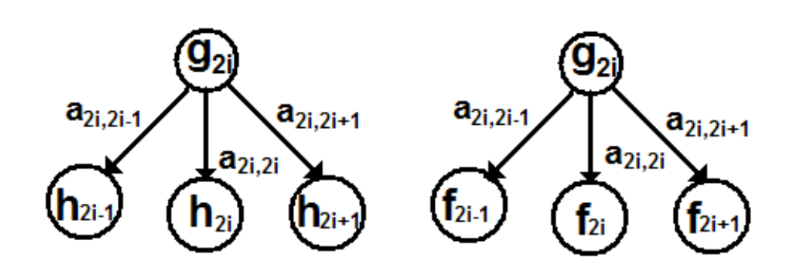
\includegraphics[scale=0.4]{difference_histogram_mtd.png}
    \end{figure}

    then, we define the following values:

    \[ \alpha_i = \frac{a_{2i+2,2i+1}}{a_{2i,2i+1}} \]
    \[ \beta_i = \frac{a_{2i+2,2i+3}}{a_{2i,2i-1}} \]
    \[ \gamma_i = \frac{g_{2i}}{g_{2i+2}} \]

    As found out by X. Ping and T. Zhang in
    \cite{new-detection-lsb-steganography}:

    \begin{itemize}
        \item if $\alpha_i \approx 1, \forall i \in \{-255, -254, ..., 255\}$
              then the image contains some hidden message;
        \item otherwise, for natural images, $\alpha_i \approx \gamma_i$ is
              satisfied.
    \end{itemize}
    
    \subsubsection{Closest Color Pair method}
    Another method used to detect hidden messages on the LSB plane is the
    \emph{Closest Color Pair method}.

    Whhen an image has a steganographed message in te LSB plane, the number of
    close colors increases \cite{detecting-lsb-steganography}. Given two pair of
    colors $C_1=[R_1,G_1,B_1],\ C_2=[R_2,G_2,B_2]$, the condition of them being
    close is:

    \[ (R_1-R_2)^2+(G_1-G_2)^2+(B_1-B_2)^2 \leq 3 \]

    We apply a LSB embedding steganography algorithm on the image and we compute
    the number of close color pairs in both images.

    Now, we define:

    \begin{itemize}
        \item $P$ as the number of close color pairs; $P'$ as the number of
              close color pairs of the stegoimage;
        \item $U$ as the number of color pairs; $U'$ as the number of color
              pairs of the stegoimage
    \end{itemize}

    Then, we compute:

    \[ R = \frac{P}{\binom{U}{2}},\ R' = \frac{P'}{\binom{U'}{2}} \]

    We know that if

    \[ \frac{R}{R'} \geq Th,\ Th = 1.1 \]

    \noindent then the image is a natural image, otherwise it contains an hidden
    message. All the proofs are in \cite{detecting-lsb-steganography}.

    \subsubsection{DCT Domain embedding method}
    The DCT Domain embedding method works on \emph{JPEG} images, one of the most
    used format on Internet web sites.
    The JPEG format uses a \emph{discrete cosine transform} (DCT) to transform
    every 8x8-pixel block into 64 DCT coefficients, that are used to calculate
    the pixels when the image is displayed.
    The DCT Domain embedding method substitute the \emph{LSB} of the
    coefficients with the secret message: since the modification is done in the
    frequency domain, there is no human perceivable change in the image.

    \subsubsection{Chi-square test}


    \subsection{Audio}
    Steganography in audio is more challenging with respect to images, because
    the \emph{human auditory system} (HAS) operates over a wide dynamic range,
    while maintaining a high sensitivity to perturbations and noises.
    Howerer, there are still some ``holes'' where data can be hidden.
    The HAS has a quite small differential range, so loud sounds mask out quiet
    sounds, moreover it is unable to perceive absolute sound phase, but only
    relative one.

    Another important factor to consider when dealing with sound are the
    transmissions enviroments.
    Audio signals can be transmitted through a digital channel (eventually being
    resampled), through an analog channel or ``over the air'' played by a
    speaker and received by a microphone.
    Depending on the transmission channel there could be huge modification that
    can make the steganalysis process impossible, but also that can compromise
    irreparably the hidden message, damaging also the steganographer.

    Due to the several issues presented above, steganalysis in audio signals is
    more complex with respect to other cover types.
    In the following sections we will cover some of the possible ways in which
    steganography and steganalysis is applied in audio signals, without entering
    too much in details.

    % Refer to data hiding to write the following subsubsection
    %   write just short paragraph explaining briefly how data are encoded and
    %   in particular how they can be retrieved
    
    \subsubsection{Low-bit coding}

    \subsubsection{Phase coding}

    \subsubsection{Spread spectrum}

    \subsubsection{Echo data hiding}
    

    \subsection{Text}
    \emph{Soft-copy text} is the most difficult place in which steganography is
    performed due to the fact that there are no redundant informations nor large
    set of data that can be slightly modified without affecting the overall look
    of the cover.
    % Read "Modern Text Hiding, Text Steganalysis, and Application"
    %   from sources folder on Drive before writing here

    \subsection{TCP/IP}
    \subsubsection{Introduction}
    Before treating such topic we must briefly discuss the behaviour of the
    TCP/IP (\textbf{Internet protocol suit}) communications.
    
    \paragraph{IP (Internet Protocol)} is at the basis of internet
    communication. The protocol exploits the principle of encapsulation, sending
    packets composed by a \emph{header} which contains information such as the
    \textbf{destination address} and \textbf{source address} and a
    \emph{payload} which represents the actual data to be transmitted.
    Since physical channels usually have a limited \emph{MTU}\footnote{Maximum
    Transmission Unit}, then the data is usually fragmented in smaller chunks,
    wrapped into an header and only then transmitted.
    
    \paragraph{TCP (Transmission Control protocol)} is a protocol used for
    reliable (little information loss), ordered, error-checked data transmission
    between a machine hosting the data (\textbf{Server}) and another requiring
    such data (\textbf{Client}). It is performed previous a three-way handshake
    which estabilishes a connection between server and client, thus preparing a
    reliable communication channel.

    \paragraph{UDP (User Datagram Protocol)}, contrary to TCP, is less reliable
    but faster.
    It broadcasts the data in an unordered and uncontrolled way to the receiver. 
    There is no need to estabilishing a connection in order to implement such
    protocol.

    \begin{figure}[h]
        \centering
        \caption{Structure of TCP packet}
        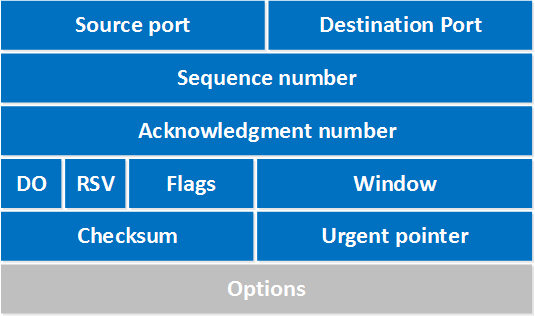
\includegraphics[scale=0.5]{tcp_header.png}
    \end{figure}

    \begin{figure}[h]
        \centering
        \caption{Structure of UDP packet}
        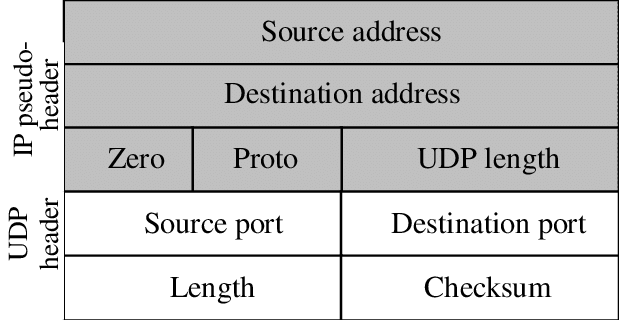
\includegraphics[scale=0.3]{udp_header.png}
    \end{figure}

    \subsubsection{Exploits and protection tools}

    As you could notice from the previous figures, the first part of the header
    is the same. This is because it is part of the IP protocol itself.
    In the second part of each header we find different types of metadata which
    are specific for each protocol. Generally the metadat contained in the
    header is redundant for the transmission of the message itself and this 
    redundancy may become a target for a \emph{stego-algorithm}\footnote{an
    algorithm used for steganography} which starting from a \emph{cover-network
    packet sequence}\footnote{a sequence of packets which will be transmitted
    over the network acting as a cover for the hidden messace} and a
    \emph{covert message}, can generate a sequence of packets(each one embedding
    a portion of the covered message) which will be sent over the network.

    This procedure is not a \emph{risk-free} approach for the attacker who
    wishes to send the \emph{cover-network packet sequence}, since it is
    possible that the data will be currupted during transmission or there could
    be losses using non-reliable transport protocols(UDP).
    Other criticalities of such method stay in the fact that the sequence of
    packets will most likely traverse multiple nodes in the network before
    reaching the target, and the message may be detected by these nodes.

    The defense against Steganography in TCP/IP communication consists in 
    series of standards which are implemented by the devices on the internet and
    that we will illustrate through some examples.


    \paragraph{Tof(Type of service)} bits are a field in the TCP header which
    are nowdays rarely used. This could open doors to a steganographic attack if
    modern operating systems did not set them to zero by default.
    A warden monitoring the channel could immediately signal an error.

    \paragraph{IP ID} is a field in the Internet Protocol which is used to
    assist the receiver in reassemblying the fragmented packets.
    This field consist of randomly unique numbers representing a packet.
    It is possible to insert other types of information in this field by simply
    conform to the uniqueness constraint.
    Since in many cases the numbers used for the IP ID are not random, by
    knowing the charachteristics of the sender it is possible to detect an
    infiltration.

    \paragraph{IP Fragment Offset} is an offset which is present in the IP
    header which helps the receiver to reconstruct the sequence of bits from the
    fragmented sequence.
    Modulating the size of the fragments changes the offset field in the header
    and thus a message could be sent.
    The protection against this method is simply checking the size of the
    packets relative to the MTU and so even in this case a warden can easily
    detect an error.

    \paragraph{TCP sequence number} is a field in the TCP header which stores
    the randomly chosen position(for security reasons) of the first byte to be
    transmitted through the channel. The steganographic method consists in
    replacing this field with the data to be sent.
    Being random it is more difficult to spot a breach in the channel.
    In this case the usage of a \emph{SVM}\footnote{Support Vector Machine}, a
    machine learning tool able to identify patterns inside the data transmitted
    could come into hand.
    However an error could be detected even simply by checking the presence of
    repetitions in the stream(not admitted by design). 

    \paragraph{Timestamp modulation} is another technique of steganography which
    operate by modifing the \emph{LSB} of the
    timestamp of a TCP packet in order to represent a '1'.
    The covert message is thus embedded into the data stream.
    Since the TCP Timestamp support is not universal, machines not supporting
    such feature may detect the hidden message.


    \subsubsection{Detection of TCP/IP steganography}

    Each operating system exhibits well defined characteristics in generated
    TCP/IP fields. These can be used to identify any anomalies that may indicate 
    the use of steganography. For this purpose, a suite of tests which may be
    applied to \emph{network traces}\footnote{function that performs network
    analysis on a geometric network} are defined and they are used to identify
    whether the results are consistent with the operating systems believed to be
    installed on the source host.
    Diffreent methods of covert channel detection are used, employing IP ID 
    characteristics, TCP ISN characteristics and explicit steganography
    detection.

    \paragraph{IP ID characteristics} are the features identifying the IP
    address, a unique address that identifies a device on the internet or local
    network. They are employed by the following methods.
    \emph{Sequential Global IP ID} implies the usage of a global counter for the
    IP ID. 
    To detect this strategy one has to look if connections to different hosts
    have sequentially increasing IP IDs.
    \emph{Sequential Per-host IP ID} is characterized by the usage of a per-host
    counter for packets. If it apperas to be fragmented, the warden can test
    whether connections to different hosts use apparently unrelated IP IDs;
    however connections to the same host have a sequentially increasing IP ID.
    \emph{IP ID MSB Toggle} represents the case where the operating system
    system toggles the most significant bit of the IP ID every rekey interval,
    so that the warden can examine the MSB to check if it matches this pattern.
    \emph{IP ID Permutation} strategy presence can be discarded by the warden if
    there are duplicates, since within a rekey interval the IP ID is
    non-repeating.

    \paragraph{Explicit steganography detection} can be employed by several
    methods.
    \emph{Nushu Criptography} is a strategy applied by Nushu, which encrypts
    data before including it in the ISN field, resulting in a distribution which
    differs form the one that is normally generated by Linux; therefore, it can
    be detected. 
    \emph{TCP Timestamp} strategy involves the execution of a randomness test.
    In particular, if a low bandwidth TCP connection is being used to leak
    information, this test can be applied to the LSBs of the timestamps in the
    TCP packets. If an excessive presence of randomness is detected in the LSBs,
    it can be deduced that a steganographic covert channel is in use.
    There are also other features which may indicate the usage of steganography:
    \emph{unsual flags}, \emph{excessive fragmentation}, use of \emph{IP
    options}, \emph{unexpected TCP options} and \emph{excessive re-ordering}.

    \pagebreak

\end{document}